% !TeX root = thesis.tex
%% content.tex
%%

%% ==============
\chapter{Algorithm}
\label{ch:Algorithm}
%% ==============
In this chapter, we introduce a labeling algorithm for the Truck Driver Routing Problem. At first, we will restrict the problem to one driving time constraint for simplicity and drop that constraint later. We then describe extensions of the base algorithm to achieve better running times on realistic problem instances.

\section{Dijkstra's Algorithm with One Driving Time Constraint\label{sec:dijkstra_csp}}
We will adapt Dijkstra's algorithm to solve the TDRP with one driving time constraint (TDRP-1DTC). While Dijkstra's algorithm manages a queue of nodes and assigns each node one tentative distance, our algorithm manages a queue $Q$ of labels and a set $L(v)$ of labels for each node $v \in V$.

Labels in a label set $L(v)$ represent a possible route, respectively a possible solution for a query from $s$ to $v$. A label $l \in L(v)$ may represent suboptimal routes to $v$, i.e., routes which are not a shortest route between $s$ and $v$. Nevertheless, we will ensure that a label set never contains labels which represent infeasible routes according to $\restr$. A label $l$ contains

\begin{itemize}
	\item $\concretett(l)$, the total travel time from the starting node $s$
	\item $\breakDist(l)$, the distance since the last break
	\item $\pred(l)$, its preceding label
\end{itemize}

As in Dijkstra's algorithm, the queue is a min-Queue with ascending keys. The key of a label $l$ is its accumulated $\traveltime(l)$.

\subsection{Settling a Label}
In contrast to Dijkstra's algorithm, the search \emph{settles} a label $l \in L(u)$ in each iteration instead of a node $u$. When settling a label, the search first removes $l$ from the queue. Similar to Dijkstra, it then relaxes all edges $(u,v) \in E$ with $l \in L(u)$ as shown in Figure~\ref{alg:settle_next_label}.

\begin{algorithm}[hbtp]
	\SetFuncSty{textsc}
	\DontPrintSemicolon
	\SetKwData{Q}{Q}
	\SetKwData{L}{L}

	\SetKwFunction{SettleNextLabel}{SettleNextLabel}
	\SetKwFunction{RelaxEdge}{RelaxEdge}
	\SetKwFunction{queueDeleteMin}{deleteMin}

	\SetKwProg{Pn}{Procedure}{:}{\KwRet}
	\Pn{\SettleNextLabel{}}{
		$l \leftarrow$ \Q.\queueDeleteMin{} \;
		\BlankLine

		\ForAll{ $(u,v) \in E$ }
		{
			\RelaxEdge{$(u,v),l$}
		}
	}
	\caption[\textsc{SettleNextLabel}]{\label{alg:settle_next_label}Settling a label $l \in L(u)$ removes the label from the queue and relaxes all the outgoing edges of $u$.}
\end{algorithm}


Relaxing an edge consists of the three steps label \emph{propagation}, \emph{pruning} and \emph{dominance} checks.

\subparagraph{Label Propagation.}
Labels can be propagated along edges. Let $l \in L(u)$ be a label at $u$ and $(u,v) = e \in E$, then $l$ can be propagated to $v$ resulting in a label $l'$ with $\concretett(l') = \concretett(l) + \mathfunction{len}(e)$, $\breakDist(l') = \breakDist(l) + \mathfunction{len}(e)$, and $\pred(l') = l$.

\subparagraph{Label Pruning.}
After propagating a label, we discard the label if it violates the driving time constraint $\restr$, that is, if $\breakDist(l) > \restr^d$.


\subparagraph{Label Dominance}
In general, it is no longer clear when a label presents a better solution than another label since it now contains two distance values. A label $l$ at a node $v$ might represent a shorter route from $s$ to $v$ than another label $l'$ but might have shorter remaining driving time budget $\restr^d - \breakDist(l)$. The label $l$ yields a better solution for a query $s$-$v$, but this does not imply that it is part of a better solution for a query from $s$-$t$. It might not even yield a feasible route to $t$ at all while $l'$ reaches the target due to the greater remaining driving time budget. In one case, we can prove that a label $l \in L(v)$ cannot yield a better solution than a label $l' \in L(v)$. We say $l'$ \emph{dominates} $l$.

\begin{definition}[Label Dominance for 1DTC]
	A label $l \in L(v)$ dominates another label $l' \in L(v)$ if $\concretett(l') > \concretett(l)$ and $\breakDist(l') \ge \breakDist(l)$ or $\concretett(l') \ge \concretett(l)$ and $\breakDist(l') > \breakDist(l)$.
\end{definition}

If a label $l \in L(v)$ is dominated by another label $l' \in L(v)$, then $l'$ represents a route from $s$ to $t$ with a shorter or equal total travel time and longer or equal remaining driving time budget until the next break. Therefore, in each solution which uses the label $l$, $l$ can trivially be replaced by the label $l'$. The solution will still comply with the driving time constraint $\restr$ and yield a shorter or equal total travel time, so we are allowed to simply discard dominated labels in our search.

\begin{definition}[Pareto-Optimal Label]
	A label $l \in L(v)$ is pareto-optimal if it is not dominated by any other label $l' \in L(v)$.
\end{definition}

A label $l$ will only be inserted into a label set $L(v)$ if it is pareto-optimal. If a label $l$ is inserted into $L(v)$, labels $l' \in L(v)$ are removed from $L(v)$ if $l$ dominates them. $L(v)$ therefore is the set of known pareto-optimal solutions at $v$. In Figure~\ref{alg:remove_dominated} we define the procedure \textsc{RemoveDominated($l$)} as an operation on a label set.

\begin{algorithm}[hbtp]
	\SetFuncSty{textsc}
	\SetKwFor{ForAll}{forall}{do}
	\DontPrintSemicolon
	\SetKwData{L}{L}

	\SetKwFunction{RemoveDominated}{RemoveDominated}
	\SetKwFunction{queueRemove}{remove}

	\SetKwProg{Pn}{Procedure}{:}{\KwRet}
	\Pn{\RemoveDominated{$l$}}{
		\ForAll{$l' \in L$}
		{
			\If{\text{$l$ dominates $l'$}}{
				\L.\queueRemove($l'$)\;
			}
		}
	}
	\caption[\textsc{RemoveDominated}]{\label{alg:remove_dominated}The procedure $L$.\textsc{RemoveDominated}($l$) removes all labels from the label set $L$ which are dominated by the label $l$.}
\end{algorithm}


\subsection{Parking at a Node}
When propagating a label $l \in L(u)$ along an edge $(u,v) \in E$ and $v \in P$, we have to consider pausing at $v$. Since we do not know if pausing at $v$ or continuing without a break is the better solution, we generate both labels and add them to the label set $L(v)$ and the queue $Q$. We now can define the procedure \textsc{RelaxEdge} as in Figure~\ref{alg:relax_edge}.

\begin{algorithm}[htbp]
	\SetFuncSty{textsc}
	\DontPrintSemicolon
	\SetKwData{Q}{Q}
	\SetKwData{L}{L}

	\SetKwFunction{RelaxEdge}{RelaxEdge}
	\SetKwFunction{queueDeleteMin}{deleteMin}

	\SetKwData{Q}{Q}
	\SetKwData{L}{L}
	\SetKwData{D}{D}
	\SetKwData{pred}{pred}
	\SetKwArray{ds}{ds}
	\SetKwFunction{queueDeleteMin}{deleteMin}
	\SetKwFunction{queueInsert}{queueInsert}
	\SetKwFunction{setInsert}{insert}
	\SetKwFunction{queueMin}{min}
	\SetKwFunction{queueMinKey}{minKey}
	\SetKwFunction{queueDecreaseKey}{decreaseKey}
	\SetKwFunction{queueContains}{contains}
	\SetKwFunction{listInsert}{insert}
	\SetKwFunction{removeDom}{RemoveDominated}

	\SetKwProg{Pn}{Procedure}{:}{\KwRet}
	\Pn{\RelaxEdge{(u,v), l}}{
		$\D \leftarrow \{\}$\;
		\If{$\breakDist(l) + \mathfunction{len}(u,v) \le \restr^d$}
		{
			\D.\setInsert{$(\concretett(l) + \mathfunction{len}(u,v), \breakDist(l) + \mathfunction{len}(u,v), l)$}\;

			\If{$v \in P$}
			{
				\D.\setInsert{$(\concretett(l) + \mathfunction{len}(u,v) + \restr^b, 0, l)$}\;
			}

			\ForAll{ $l' \in D$ }
			{
				\If{$l'$ is not dominated by any label in \L{$v$}}
				{
					\L{$v$}.\removeDom{$l'$} \;
					\L{$v$}.\setInsert{$l'$} \;
					\Q.\queueInsert{$\concretett(l')$,$l'$}
				}
			}
		}
	}
	\caption[\textsc{RelaxEdge}]{\label{alg:relax_edge}Relaxing an edge $(u,v) \in E$ when settling a label $l \in L(u)$ with regard to parking nodes.}
\end{algorithm}

\subsection{Initialization and Main Loop}
We initialize the label set $L(s)$ of $s$ and the queue $Q$ with a label which only contains distances of zero and a dummy element as a predecessor. We stop the search when $t$ was removed from $Q$. The definition of the final algorithm is given as Algorithm~\ref{alg:CSP} \textsc{Dijkstra+1DTC}.

\begin{algorithm}[htbt]
	\caption{\textsc{Dijkstra for TDRP-1DTC}}\label{alg:CSP}

	% Some settings
	\DontPrintSemicolon %dontprintsemicolon
	\SetFuncSty{textsc}
	\SetKwFor{ForAll}{forall}{do}

	% Declaration of data containers and functions
	\SetKwData{Q}{Q}
	\SetKwData{dist}{d}
	\SetKwData{L}{L}
	\SetKwData{pred}{pred}
	\SetKwArray{ds}{ds}
	\SetKwFunction{queueDeleteMin}{deleteMin}
	\SetKwFunction{queueInsert}{queueInsert}
	\SetKwFunction{setInsert}{insert}
	\SetKwFunction{queueMin}{min}
	\SetKwFunction{queueMinKey}{minKey}
	\SetKwFunction{queueDecreaseKey}{decreaseKey}
	\SetKwFunction{queueContains}{contains}
	\SetKwFunction{listInsert}{insert}
	\SetKwFunction{removeDom}{RemoveDominated}
	\SetKwFunction{SettleNextLabel}{SettleNextLabel}

	% Algorithm interface
	\KwIn{Graph $G=(V,E,\mathfunction{len})$, set of parking nodes $P \subseteq V$, set of driving time constraints $\restrset=\{r\}$, start and target nodes $s,t \in V$}
	\KwData{Priority queue \Q, per node set \L{$v$} of labels for all $v \in V$}
	\KwOut{Shortest route with $\concretett(j) = \traveltime(s,t)$}

	% The algorithm
	\BlankLine
	\tcp{Initialization}
	\Q.\queueInsert{$0$,$(0,0,\bot)$}\;
	\L{$s$}.\setInsert{$(0,0,\bot)$}\;
	\BlankLine
	\tcp{Main loop}
	\While{\Q is not empty}
	{
		\SettleNextLabel{}\;

		\If{\text{label at $t$ was settled}}
		{
			\Return\;
		}
	}
\end{algorithm}

\subsection{Correctness\label{sec:dijkstra_csp_correctness}}
Given a start node $s$ and a target node $t$, Dijkstra's algorithm returns the shortest distance between $s$ and $t$. The algorithm can be stopped after $t$ was removed from the queue since all the following nodes in the queue have larger distances and the edge lengths are non-negative by definition. Therefore, relaxing an outgoing edge of these nodes cannot lead to an improvement of the distance at $t$.

In our case, the algorithm shall return the shortest travel time $\traveltime(s,t)$ between two nodes $s$ and $t$. We have a queue of labels which is sorted in ascending order by their travel time. When removing a label $l$ from the queue, all the other labels in the queue therefore have a larger travel time than $\concretett(l)$. Additionally, all the edge lengths and the break times are non-negative. Relaxing an edge thus can only increase the travel time. The same argument as for the correctness of Dijkstra's algorithm applies: Since relaxing an edge can only increase travel time, labels which are added later to the queue will also have a larger travel time than $\concretett(l)$. Therefore, when we remove the first label $l_t \in L(t)$ at $t$ from the queue, we know that this time cannot be improved further and it is correct to stop the search.

When relaxing an edge $(u,v)$ and propagating a label $l \in L(u)$, we check if the new label complies with the driving time constraints. We do not insert the new label into $L(v)$ and the queue if it violates a constraint. Therefore, label sets and the queue only contain labels which represent a feasible route and $l_t$ must also represent a feasible route.

If we propagated a label to a parking node, we produce a second label since we have the two choices of parking and not parking at the node. We treat both labels equally and insert both labels into label set and queue if they are not dominated or represent an infeasible route. The label with the smaller travel time will be removed first from the queue, and the second label will be handled at a later stage when its travel time becomes the smallest of all labels in the queue. It is not possible to miss possible routes between $s$ and $t$ because we produce all the labels and only discard dominated labels and labels representing infeasible routes. There therefore cannot be a label with a better travel time from $s$ to $t$ than the label $l_t$ which we removed as the first label at t from the queue. Therefore, its travel time $\concretett(l_t)$ is equal to the shortest travel time $\traveltime(s,t)$ between $s$ and $t$.

\section{Goal-Directed Search with One Driving Time Constraint}
In this section, we extend the base algorithm described in Section~\ref{sec:dijkstra_csp} to a goal-directed search with the A* algorithm. We introduce a new potential $\concretepotential_t$ based on the CH-Potentials in Section~\ref{sec:ch_pot}. We then show that we still can stop the search when the first label at $t$ is removed from the queue.

The difference between Dijkstra and A* is the order in which nodes are being removed from the queue. In our case, this corresponds to the order of labels being removed from the queue. Instead of using their travel time $\concretett(l)$ as a queue key, a label $l \in L(v)$ is added to the queue with the key $\concretett(l) + \concretepotential_t(l,v)$. Algorithm~\ref{alg:CSPPot} shows the adaption of the coarse algorithm.

\begin{algorithm}[bt]
	\caption{\textsc{A* for TDRP-1DTC}}\label{alg:CSPPot}

	% Some settings
	\DontPrintSemicolon %dontprintsemicolon
	\SetFuncSty{textsc}
	\SetKwFor{ForAll}{forall}{do}

	% Declaration of data containers and functions
	\SetKwData{Q}{Q}
	\SetKwData{dist}{d}
	\SetKwData{L}{L}
	\SetKwData{pred}{pred}
	\SetKwArray{ds}{ds}
	\SetKwFunction{queueDeleteMin}{deleteMin}
	\SetKwFunction{queueInsert}{queueInsert}
	\SetKwFunction{setInsert}{insert}
	\SetKwFunction{queueMin}{min}
	\SetKwFunction{queueMinKey}{minKey}
	\SetKwFunction{queueDecreaseKey}{decreaseKey}
	\SetKwFunction{queueContains}{contains}
	\SetKwFunction{listInsert}{insert}
	\SetKwFunction{removeDom}{RemoveDominated}
	\SetKwFunction{settleNextNode}{settleNextNode}

	% Algorithm interface
	\KwIn{Graph $G=(V,E,\mathfunction{len})$, set of parking nodes $P \subseteq V$, a set of driving time constraints $\restrset = \{r\}$, start and target nodes $s,t \in V$, potential $\concretepotential_t()$}
	\KwData{Priority queue \Q, per node set \L{$v$} of labels for all $v \in V$}
	\KwOut{Shortest route with $\concretett(j) = \traveltime(s,t)$}

	% The algorithm
	\BlankLine
	\tcp{Initialization}
	$l_s \leftarrow (0,0,\bot)$\;
	\Q.\queueInsert{$\concretepotential_t((l_s),s)$, $l_s$}\;
	\L{$s$}.\setInsert{$l_s$}\;
	\BlankLine
	\tcp{Main loop}
	\While{\Q is not empty}
	{
		\settleNextNode{}\;

		\If{\text{minimum of $Q$ is label at $t$}}
		{
			\Return\;
		}
	}
\end{algorithm}

The only thing left is the adaption of \textsc{RelaxEdge} in Figure~\ref{alg:relax_edge} where we change the queue keys to use $\concretett(l) + \concretepotential(l,v)$ instead. The result is shown in Figure~\ref{alg:relax_edge_a_star}.

\begin{algorithm}[hbtp]
	\SetFuncSty{textsc}
	\DontPrintSemicolon
	\SetKwData{Q}{Q}
	\SetKwData{L}{L}

	\SetKwFunction{RelaxEdge}{RelaxEdge}
	\SetKwFunction{queueDeleteMin}{deleteMin}

	\SetKwData{Q}{Q}
	\SetKwData{L}{L}
	\SetKwData{D}{D}
	\SetKwData{pred}{pred}
	\SetKwArray{ds}{ds}
	\SetKwFunction{queueDeleteMin}{deleteMin}
	\SetKwFunction{queueInsert}{queueInsert}
	\SetKwFunction{setInsert}{insert}
	\SetKwFunction{queueMin}{min}
	\SetKwFunction{queueMinKey}{minKey}
	\SetKwFunction{queueDecreaseKey}{decreaseKey}
	\SetKwFunction{queueContains}{contains}
	\SetKwFunction{listInsert}{insert}
	\SetKwFunction{removeDom}{RemoveDominated}

	\SetKwProg{Pn}{Procedure}{:}{\KwRet}
	\Pn{\RelaxEdge{$(u,v)$, $l$}}{
		$\D \leftarrow \{\}$\;
		\If{$\breakDist(l) + \mathfunction{len}(u,v) \le \restr^d$}
		{
			\D.\setInsert{$(\concretett(l) + \mathfunction{len}(u,v), \breakDist(l) + \mathfunction{len}(u,v), l)$}\;

			\If{$v \in P$}
			{
				\D.\setInsert{$(\concretett(l) + \mathfunction{len}(u,v) + \restr^b, 0, l)$}\;
			}

			\ForAll{ $l' \in D$ }
			{
				\If{$l'$ is not dominated by any label in \L{$v$}}
				{
					\L{$v$}.\removeDom{$l'$} \;
					\L{$v$}.\setInsert{$l'$} \;
					\Q.\queueInsert{$\concretett(l') + \concretepotential_t(l',v)$, l'}
				}
			}
		}
	}
	\caption[\textsc{RelaxEdge} with potential]{\label{alg:relax_edge_a_star} Relaxing an edge with regard to the potential.}
\end{algorithm}

\subsection{Potential for One Driving Time Constraint}\label{section:potential_csp}
In general, every feasible potential can be used for the goal-directed algorithm. We use CH-Potentials as foundation to build a potential which accounts for necessary break times on the route.

Given a target node $t$, the CH-Potentials yield a perfect estimate for the distance $\distance(v,t)$ from $v$ to $t$ without regard for driving time constraints and breaks. This is a lower bound for the remaining travel time for any label at $v$. A better lower bound for the remaining travel time of a label at $v$ to $t$, including breaks due to the driving time limit, can be calculated by taking the minimum necessary amount of breaks into account. We define \minBreaks($d$) as a function of time which calculates the minimum amount of necessary breaks for any arbitrary driving time $d$.

\begin{align}\label{eq:min_breaks}
	\minBreaks(d) = \begin{dcases}
		\ceil*{ \frac{d}{\restr^d} } - 1 & d > 0 \\
		0                                & else
	\end{dcases}
\end{align}

Simply using $\floor*{ \frac{d}{\restr^d} }$ is not sufficient since we do not need to pause for a driving time of exactly $\restr^d$. We now can calculate a lower bound for the minimum necessary break time given an arbitrary driving time $d$

\begin{align}\label{eq:min_break_time}
	\minBreakTime(d) = \minBreaks(d) \cdot \restr^b
\end{align}

and finally define our node potential as

\begin{align}
	\begin{split}
		\concretepotential{'}_t(v) & = \minBreakTime(\chpotential_t(v)) + \chpotential_t(v)
	\end{split}
\end{align}

A node potential is called \emph{feasible} if it does not overestimate the distance of any edge in the graph, i.e.

\begin{align}
	\label{eq:node_potential_feasibility}
	len(u,v) - \concretepotential_t(u) + \concretepotential_t(v) \ge 0 \quad \forall (u,v) \in E
\end{align}

A feasible node potential allows us to stop the A* search when the node $t$, respectively the first label at $t$, was removed from the queue. Following counterexample of a query using the graph in Fig.~\ref{fig:graph_infeasible_potential} shows that $\concretepotential{'}_t$ is not feasible. With a driving time limit of 6 and a break time of 1, the potential here will yield a value $\concretepotential_t(s) = 8$ since the potential includes the minimum required break time for a path from s to t. Consequently, with $\concretepotential{'}_t(v) = 5$ and $len(s,v) = 2$, $len(s,v) - \concretepotential{'}_t(s) + \concretepotential{'}_t(v) = -1$.

\begin{figure}[hbtp]
	\centering
	\tikzstyle{node}=[circle,inner sep=0.5mm,minimum size=5.25mm,draw = black]
\tikzstyle{bright}=[fill=black!14]
\tikzstyle{dark}=[fill=black!28]
\tikzstyle{lightEdgeStyle}=[black!20]

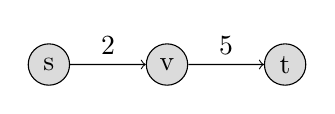
\begin{tikzpicture}[scale=1.5, bend angle = 20]

	% Obere Reihe
	\node(s) at (1,1) [node, bright] {s};
	\node(v) at (2,1) [node, bright] {v};
	\node(t) at (3,1) [node, bright] {t};

	\draw[->] (s) -> node[midway, above]{2} (v);
	\draw[->] (v) -> node[midway, above]{5} (t);
	% \foreach \i [evaluate = \i as \lastNode using \i-1] in {2,3,...,\numberOfNodes}
	% 	{
	% 		\node (Top\i) at (\i,1) [node, bright] {\i}
	% 		edge[<-] (Top\lastNode);
	% 	}


	% % Pfeile nach rechts
	% \pgfmathparse{\numberOfNodes - 2}
	% \foreach \i [evaluate = \i as \nextNode using \i+2] in {1,2,...,\pgfmathresult}
	% 	{
	% 		\foreach \j [count=\nodeIndex from \nextNode] in {\nextNode,...,\numberOfNodes}
	% 			{
	% 				\draw[->, lightEdgeStyle] (Bot\i) to [bend right] (Bot\nodeIndex);
	% 			}
	% 	}

\end{tikzpicture}

	\caption{Example graph for which the feasibility condition of~\ref{eq:node_potential_feasibility} does not always hold with the potential $\concretepotential'$.}
	\label{fig:graph_infeasible_potential}
\end{figure}

A variant of the potential accounts for the distance since the last break of a label $\breakDist(l)$ to calculate the minimum required break time on the $v$-$t$ path.

\begin{align}
	\begin{split}
		\concretepotential_t(l,v) & = \minBreakTime(\breakDist(l) + \chpotential_t(v)) +\chpotential_t(v)
	\end{split}
\end{align}

Since the potential now uses information from a label $l$ with $l \in L(v)$, it no longer is a node potential but also depends on the chosen label at $v$. The feasibility definition as defined in~\ref{eq:node_potential_feasibility} can no longer be applied. We therefore have to show that queue keys of labels can only increase over time.

\begin{lemma}\label{lemma:pot_labels_get_larger}
	Let $l$ be a label in the label set $L(u)$ which the algorithm propagates along the edge $(u,v) \in E$ to create a label $l' \in L(v)$. The sum of travel time and potential of a label can only increase, i.e, $\concretett(l) + \concretepotential_t(l,u) \le \concretett(l') + \concretepotential_t(l',v)$.
\end{lemma}

\begin{proof}
	Let $(u,v) \in E$ be an edge. The procedure \textsc{RelaxEdge} in Figure~\ref{alg:relax_edge_a_star} can produce two new labels at a node $v$ for each label at $u$, depending on if $v$ is a parking node. We differentiate the two cases not parking at $v$ and parking at $v$. Let $l \in L(u)$ and $l' \in L(v)$.

	Following general observations can be made:

	\begin{enumerate}
		\item $d \ge d' \implies \minBreakTime(d) \ge \minBreakTime(d')$
		\item $\restr^b + \minBreakTime(d) \ge \minBreakTime(d + \restr^d)$
		\item $\restr^d \ge \breakDist(l') \ge \breakDist(l) + \len(u,v) \ge \breakDist(l)$\\(Line $2$ in \textsc{RelaxEdge} in Figure~\ref{alg:relax_edge_a_star})
		\item   $\len(u,v) - \chpotential_t(u)+ \chpotential_t(v) \ge 0$ (feasibility of the CH-Potentials)
		\item  $\len(u,v) + \chpotential_t(v) \ge \chpotential_t(u)$
	\end{enumerate}

	We show that $\concretett(l') + \concretepotential_t(l',v) - \concretett(l) - \concretepotential_t(l,u) \ge 0$.

	\emph{Case 1: Not parking at $v$.} In this case, $\concretett(l') = \concretett(l) + \len(u,v)$ and $\breakDist(l') = \breakDist(l) + \len(u,v)$.

	\begin{align}
		\begin{split}\label{eq:label_feasibility_proof_1}
			&\concretett(l') - \concretett(l) - \concretepotential_t(l,u) + \concretepotential_t(l',v)\\
			&= \concretett(l) + \len(u,v) - \concretett(l)\\
			& \phantom{{}=1} - (\minBreakTime(\breakDist(l)+\chpotential_t(u)) + \chpotential_t(u))\\
			& \phantom{{}=1} + \minBreakTime(\breakDist(l')+\chpotential_t(v)) + \chpotential_t(v)\\
			&= \len(u,v) + \minBreakTime(\breakDist(l')+\chpotential_t(v))\\
			& \phantom{{}=1} - \minBreakTime(\breakDist(l)+\chpotential_t(u)) - \chpotential_t(u) + \chpotential_t(v)\\
			&= \len(u,v) + \minBreakTime(\breakDist(l) + \len(u,v) + \chpotential_t(v))\\
			& \phantom{{}=1} - \minBreakTime(\breakDist(l)+\chpotential_t(u)) - \chpotential_t(u) + \chpotential_t(v) \\
			\overset{\text{(1. and 5.)}}&{\ge} \len(u,v) + \minBreakTime(\breakDist(l) + \chpotential_t(u))\\
			& \phantom{{}=1} - \minBreakTime(\breakDist(l)+\chpotential_t(u)) - \chpotential_t(u) + \chpotential_t(v) \\
			&= \len(u,v) - \chpotential_t(u) + \chpotential_t(v)\\
			\overset{\text{(4.)}}&{\ge} 0
		\end{split}
	\end{align}

	\emph{Case 2: Parking at $v$.} In this case, $\concretett(l') = \concretett(l) + \len(u,v) + \restr^b$ and $\breakDist(l') = 0$.

	\begin{align}
		\begin{split}\label{eq:label_feasibility_proof_2}
			&\concretett(l') - \concretett(l) - \concretepotential_t(l,u) + \concretepotential_t(l',v)\\
			&= \concretett(l) + \len(u,v) + \restr^b - \concretett(l)\\
			& \phantom{{}=1} - (\minBreakTime(\breakDist(l) + \chpotential_t(u)) + \chpotential_t(u))\\
			& \phantom{{}=1} + \minBreakTime(\chpotential_t(v)) + \chpotential_t(v)\\
			&=  \len(u,v) + \restr^b + \minBreakTime(\chpotential_t(v))\\
			& \phantom{{}=1} - \minBreakTime(\breakDist(l)+\chpotential_t(u)) - \chpotential_t(u) + \chpotential_t(v)\\
			\overset{\text{(2.)}}&{\ge}  \len(u,v) + \minBreakTime(\restr^d + \chpotential_t(v))\\
			& \phantom{{}=1} - \minBreakTime(\breakDist(l)+\chpotential_t(u)) - \chpotential_t(u) + \chpotential_t(v)\\
			\overset{\text{(1. and 3.)}}&{\ge} \len(u,v) + \minBreakTime(\breakDist(l) + \len(u,v) + \chpotential_t(v))\\
			& \phantom{{}=1} - \minBreakTime(\breakDist(l)+\chpotential_t(u)) - \chpotential_t(u) + \chpotential_t(v)\\
			\overset{\text{(1. and 4.)}}&{\ge} \len(u,v) + \minBreakTime(\breakDist(l) + \chpotential_t(u))\\
			& \phantom{{}=1} - \minBreakTime(\breakDist(l)+\chpotential_t(u)) - \chpotential_t(u) + \chpotential_t(v)\\
			&=  \len(u,v) - \chpotential_t(u) + \chpotential_t(v)\\
			\overset{\text{(4.)}}&{\ge} 0
		\end{split}
	\end{align}
\end{proof}

\begin{lemma}\label{lemma:pot_lower_bound_csp}
	The sum $\concretett(l) + \concretepotential_t(l,v)$ of a label $l$ at a node $v$ is a lower bound for the travel time from $s$ to $t$ of the route using $l$.
\end{lemma}

\begin{proof}
	Let $r$ be a route between $s$ and $t$ with the path $p = \langle s=v_0,v_1,\ldots,t=v_k \rangle$. The route is represented by labels $l_i$ at nodes $v_i$. With Lemma~\ref{lemma:pot_labels_get_larger} and $\concretepotential_t(l_k,v_k) = 0$ follows

	\begin{align*}
		\concretett(l_{i}) + \concretepotential_t(l_{i},v_{i}) & \le \concretett(l_{i+1}) + \concretepotential_t(l_{i+1},v_{i+1})     \\
		                                                       & \le \dots \le \concretett(l_{k}) + \concretepotential_t(l_{k},v_{k}) \\
		                                                       & = \concretett(l_k) = \concretett(r)
	\end{align*}
\end{proof}

\begin{theorem}\label{theorem:pot_stop_criterion}
	The search can be stopped when the first label at $t$ is removed from the queue.
\end{theorem}

\begin{proof}
	Let $l_t$ be the first label at $t$ which is removed from the queue during an $s$-$t$ query. It represents a route $r$ from $s$ to $t$ with a travel time of  $\concretett(r) = \concretett(l_t)$. When the label $l_t$ is removed from the queue, all remaining labels $l$ at nodes $v$ in the queue fulfill $\concretett(l) + \concretepotential_t(l,v) \ge \concretett(l_t) + \concretepotential_t(l_t,t)$. The same holds for all labels which will be inserted into the queue at a later point in time (Lemma~\ref{lemma:pot_labels_get_larger}). Assume for contradiction that $r$ is not the shortest possible route from $s$ to $t$. Then, a shorter route $r'$ exists which uses at least one unsettled label $l \in L(v)$ at a node $v$. The label $l$ is eventually propagated to $t$ where a label $l_t' \in L(t)$ is created to represent the route $r'$. With Lemmas~\ref{lemma:pot_labels_get_larger}, \ref{lemma:pot_lower_bound_csp}, and $\concretepotential_t(l_t,t) = 0$ follows

	\begin{align}
		\begin{split}
			\concretett(r) = \concretett(l_t) &= \concretett(l_t) + \concretepotential_t(l_t,t) \\
			\overset{\text{(\ref{lemma:pot_labels_get_larger})}}&{\le} \concretett(l) + \concretepotential_t(l,v)\\
			\overset{\text{(\ref{lemma:pot_lower_bound_csp})}}&{\le} \concretett(l_t') = \concretett(r')
		\end{split}
	\end{align}

	which contradicts the assumption that $r'$ yields a shorter $s$-$t$ route than $r$. Therefore, it must be $\concretett(r) = \traveltime(s,t)$ when $l_t$ was removed from the queue. The search can be stopped when the first label at $t$ is removed from the queue.
\end{proof}

\section{Multiple Driving Time Constraints\label{section:n_csp}}
Dijkstra's algorithm for the Truck Driver Routing PRoblem with one driving time constraint (TDRP-1DTC) can be adapted to handle multiple driving time constraints $\restr_i$ (TDRP-mDTC). With a number of $|\restrset|$ driving time constraints, a label $l$ now contains the total travel time $\concretett(l)$ and $|C|$ distances $\breakDist_1(l), \ldots , \breakDist_{|C|}(l)$. Each value $\breakDist_i(l)$ represents the distance since the last break at a node $v$ with break time $\breakTime(v) \ge \restr_i^b$. Pausing at a node occurs with one of the available break times $\restr_i^b$ of a driving time constraint $\restr_i \in \restrset$. Pausing with an arbitrary break time is permitted but yields longer travel times and no advantage and is therefore ignored. When a route breaks at $v$ for a time $\restr_i^b$, the corresponding label $l \in L(v)$ has $\breakDist(l) = 0$ for all $0 < j \le i$ since the breaks with shorter break times are included in the longer break. In the following, we redefine the fundamental concepts of Section~\ref{sec:dijkstra_csp} for multiple driving time constraints.

\subparagraph{Label Propagation}
Label propagation simply extends the component-wise addition of the edge weight. Let $l \in L(u)$ be a label at $u$ and $(u,v) = e \in E$, then $l$ can be propagated to $v$ resulting in a label $l'$ with $\concretett(l') = \concretett(l) + \mathfunction{len}(e)$, $\breakDist_i(l') = \breakDist_i(l) + \mathfunction{len}(e)$ $\forall\ 1 \le i \le |\restrset|$, and $\pred(l') = l$.

\subparagraph{Label Pruning}
The pruning rule for driving time constraints is generalized in a similar way. A label is discarded if $\breakDist_i(l) > \restr_i^d$ for any $i$ with $0 < i \le |\restrset|$.


\subparagraph{Label Dominance}
Label dominance can be generalized to multiple driving time constraints as follows.

\begin{definition}[Label Dominance]
	A label $l \in L(v)$ dominates another label $l' \in L(v)$ if $\concretett(l') \ge \concretett(l)$ and $\breakDist_i(l') \ge \breakDist_i(l)$ $\forall\ 1 \le i \le |\restrset|$.
\end{definition}

\subsection{Potential for Multiple Driving Time Constraints\label{section:potential_n_csp}}
TODO: Rewrite for only two dtc?

In Section~\ref{section:potential_csp} we defined the potential $\concretepotential_t(l,v)$ to extend Dijkstra's algorithm with one driving time constraint to a goal-directed search using the A* algorithm. We will now generalize $\concretepotential_t$ for the use with an arbitrary number of driving time constraints.

In Equation~\refeq{eq:min_breaks} we used the distance $\distance(v,t)$ without regard for pausing from $v$ to $t$ and the distance $\breakDist(l)$ since the last break on the route to calculate a lower bound for the amount of necessary breaks until we reach the target node. We now have to calculate the lower bound with respect to all driving time constraints. How many breaks of which duration do we need at least to comply with all driving time constraints $\restr_i$? For longer driving time constraints, we will always need a greater or equal amount of breaks than for shorter driving time constraints since they have a longer maximum allowed driving time $\restr_i^d$. At the same time, a break of length $\restr_i^b$ will also include breaks of lengths $\restr_j^b$ with $j < i$. We start with calculating the amount of necessary breaks $\minBreaks_i(d)$, given a driving time $d$, for all constraints $\restr_i$ independently.

\begin{align}\label{eq:min_breaks_n}
	\minBreaks_i(d) = \begin{dcases}
		\ceil*{ \frac{d}{\restr_i^d} } - 1 & d > 0 \\
		0                                  & else
	\end{dcases}
\end{align}

Consider the example graph in Figure~\ref{fig:graph_short_long_break} with two driving time constraints with permitted driving times of $4$ and $9$. Since the distance $\distance(s,t)$ is $10$, a route must have at least one long and two short breaks. If the long break is made at $u$, only one additional short break must be made at $w$. The long break made one shorter break obsolete. To obtain a lower bound for the amount of breaks for a constraint $\restr_i$, we therefore must subtract the minimum amount of longer breaks being made on the route.

\begin{figure}[hbtp]
	\centering
	\tikzstyle{node}=[circle,inner sep=0.5mm,minimum size=5.25mm,draw = black]
\tikzstyle{bright}=[fill=black!14]
\tikzstyle{dark}=[fill=black!28]
\tikzstyle{lightEdgeStyle}=[black!20]

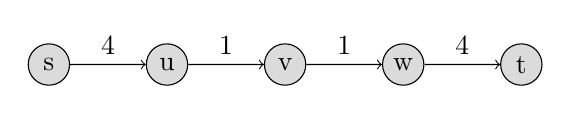
\begin{tikzpicture}[scale=1.5, bend angle = 20]

	% Obere Reihe
	\node(s) at (1,1) [node, bright] {s};
	\node(u) at (2,1) [node, bright] {u};
	\node(v) at (3,1) [node, bright] {v};
	\node(w) at (4,1) [node, bright] {w};
	\node(t) at (5,1) [node, bright] {t};

	\draw[->] (s) -> node[midway, above]{4} (u);
	\draw[->] (u) -> node[midway, above]{1} (v);
	\draw[->] (v) -> node[midway, above]{1} (w);
	\draw[->] (w) -> node[midway, above]{4} (t);
	% \foreach \i [evaluate = \i as \lastNode using \i-1] in {2,3,...,\numberOfNodes}
	% 	{
	% 		\node (Top\i) at (\i,1) [node, bright] {\i}
	% 		edge[<-] (Top\lastNode);
	% 	}


	% % Pfeile nach rechts
	% \pgfmathparse{\numberOfNodes - 2}
	% \foreach \i [evaluate = \i as \nextNode using \i+2] in {1,2,...,\pgfmathresult}
	% 	{
	% 		\foreach \j [count=\nodeIndex from \nextNode] in {\nextNode,...,\numberOfNodes}
	% 			{
	% 				\draw[->, lightEdgeStyle] (Bot\i) to [bend right] (Bot\nodeIndex);
	% 			}
	% 	}

\end{tikzpicture}

	\caption{Example graph where a long break at can render a short break obsolete.}
	\label{fig:graph_short_long_break}
\end{figure}

This is an optimistic assumption since not in all cases a longer break spares a shorter break. Revisit the example graph of Figure~\ref{fig:graph_short_long_break} with permitted driving times of $4$ and $5$. We still need one long and two short breaks, but the long break now must take place at $v$ while the short breaks must take place at $u$ and $w$. The long break did not spare a short break. Since we are searching for a lower bound for the amount of breaks, optimistic assumptions are necessary. Given a label $l \in L(v)$, the lower bound estimate for the remaining number of breaks of length $\restr_i^b$ on the route to $t$ then becomes

\begin{align}\label{eq:number_breaks_sum}
	\breakEstimate_i(l,v)  =\begin{dcases}
		\parbox[t]{.55\textwidth}{$\minBreaks_i(\breakDist_i(l) + \chpotential_t(v))$ \\\phantom{{}=1}$- \sum_{j=i+1}^{|C|}{\breakEstimate_j(l,v)}$} & 0 < i < |C| \\
		\minBreaks_{|C|}(\breakDist_{|C|}(l) + \chpotential_t(v)) & i=|C|
	\end{dcases}
\end{align}

Since we subtract all break estimates for break times greater than $\restr_i^b$ to obtain the estimate for $\restr_i^b$, we can just use

\begin{align}\label{eq:break_estimate_n}
	\breakEstimate_i(l,v) = \begin{dcases}
		\parbox[t]{.55\textwidth}{$\minBreaks_i(\breakDist_i(l) + \chpotential_t(v))$ \\\phantom{{}=1}$- \minBreaks_{i+1}(\breakDist_{i+1}(l) + \chpotential_t(v))$} & 0 < i < |C| \\
		\minBreaks_{|C|}(\breakDist_{|C|}(l) + \chpotential_t(v)) & i=|C|
	\end{dcases}
\end{align}

We now can calculate a lower bound estimate for the remaining necessary break time on the route to $t$ for two driving time constraints.

\begin{align}\label{eq:rem_break_time_n}
	\begin{split}
		\remBreak(l,v) & = \sum_{i=1}^{|C|}{\breakEstimate_i(l,v)} \cdot \restr_i^b
	\end{split}
\end{align}

Finally, the lower bound potential for a label $l \in L(v)$ and a target node $t$ becomes

\begin{align}\label{eq:multiple_breaks_pot}
	\begin{split}
		\concretepotential_t(l,v) & =\remBreak(l,v) + \chpotential_t(v,t)
	\end{split}
\end{align}

If queue keys still cannot decrease when propagating labels, Lemma~\ref{lemma:pot_lower_bound_csp} and theorem~\ref{theorem:pot_stop_criterion} follow as a consequence. We follow the outLine of the proof of Lemma~\ref{lemma:pot_labels_get_larger} and therefore revisit the procedure \textsc{RelaxEdge} at an edge $(u,v) \in E$ with a label $l \in L(u)$ and a new label $l' \in L(v)$.

\begin{lemma}\label{lemma:pot_labels_get_larger_n}
	Lemma~\ref{lemma:pot_labels_get_larger} still holds for two driving time constraints.
\end{lemma}

\begin{proof}
	There now are three cases to differentiate: not parking at $v$, short break at $v$, and long break at $v$.

	Following general observations can be made in an addition to the proof of Lemma~\ref{lemma:pot_labels_get_larger}:

	\begin{enumerate}
		\setcounter{enumi}{5}
		\item $d \ge d' \implies \minBreaks_i(d) \ge \minBreaks_i(d')$ (adaption of 1.)
		\item $1 + \minBreaks_i(d) \ge \minBreaks_i(d + \restr_i^d)$ (adaption of 2.)
		\item $\restr_i^d \ge \breakDist_i(l') \ge \breakDist_i(l) + \len(u,v) \ge \breakDist_i(l)$ (adaption of 3.)
		      % \item Propagating a label $l \in L(u)$ to obtain a label $l' \in L(v)$ $\implies$ $\remBreak(l',v) \ge \remBreak(l,u)$ (6. and non-negative edge weights)
		      % \item $d \ge d' \implies \breakEstimate(d) \ge \breakEstimate(d')$
		      % \item $\breakEstimate_i(d + \restr_i^d) \ge \restr_i^b + \breakEstimate_i(d)$ (adaption of 2.)
		      % \item $\restr_i^d \ge \breakDist_i(l') \ge \breakDist_i(l) + \len(u,v) \ge \breakDist_i(l)$ (adaption of 3.)
		      % \item Propagating a label $l \in L(u)$ to obtain a label $l' \in L(v)$ $\implies$ $\remBreak(l',v) \ge \remBreak(l,u)$ (6. and 7.)
	\end{enumerate}

	\emph{Case 1: Not parking at $v$}. In this case, $\concretett(l') = \concretett(l) + \len(u,v)$ and $\breakDist_i(l') = \breakDist_i(l) + \len(u,v)$.

	\begin{align}
		\begin{split}\label{eq:label_n_feasibility_proof_1}
			&\concretett(l') - \concretett(l) - \concretepotential_t(l,u) + \concretepotential_t(l',v)\\
			&= \concretett(l) + \len(u,v) - \concretett(l)\\
			& \phantom{{}=1} - (\remBreak(l,u) + \chpotential_t(u)) + (\remBreak(l',v) + \chpotential_t(v))\\
			&= \len(u,v) - \remBreak(l,u) + \remBreak(l',v) - \chpotential_t(u) + \chpotential_t(v)\\
			&= \len(u,v) + \breakEstimate_2(l',v) \cdot \restr_2^b + \breakEstimate_1(l',v) \cdot \restr_1^b\\
			& \phantom{{}=1} - \remBreak(l,u) - \chpotential_t(u) + \chpotential_t(v)\\
			&= \len(u,v) + \minBreaks_2(\breakDist_2(l) + \len(u,v) + \chpotential_t(v)) \cdot \restr_2^b\\
			& \phantom{{}=1} + (\minBreaks_1(\breakDist_1(l) + \len(u,v) + \chpotential_t(v))\\
			& \phantom{{}=1} - \minBreaks_2(\breakDist_2(l) + \len(u,v) + \chpotential_t(v))) \cdot \restr_1^b\\
			& \phantom{{}=1} - \remBreak(l,u) - \chpotential_t(u) + \chpotential_t(v)\\
			\overset{\text{(5. and 6.)}}&{\ge} \len(u,v)  + \minBreaks_2(\breakDist_2(l) + \chpotential_t(u)) \cdot \restr_2^b\\
			& \phantom{{}=1} + (\minBreaks_1(\breakDist_1(l) + \chpotential_t(u))\\
			& \phantom{{}=1} - \minBreaks_2(\breakDist_2(l) + \chpotential_t(u))) \cdot \restr_1^b\\
			& \phantom{{}=1} - \remBreak(l,u) - \chpotential_t(u) + \chpotential_t(v)\\
			&= \len(u,v) +  \remBreak(l,u) - \remBreak(l,u) - \chpotential_t(u) + \chpotential_t(v)\\
			&= \len(u,v) - \chpotential_t(u) + \chpotential_t(v)\\
			\overset{\text{(4.)}}&{\ge} 0
		\end{split}
	\end{align}

	\emph{Case 2: Short break at $v$}. In this case, $\concretett(l') = \concretett(l) + \len(u,v) + \restr^b$ and $\breakDist_1(l') = 0$ and $\breakDist_2(l') = \breakDist_2(l) + \len(u,v)$.

	\begin{align}
		\begin{split}\label{eq:label_n_feasibility_proof_2}
			&\concretett(l') - \concretett(l) - \concretepotential_t(l,u) + \concretepotential_t(l',v)\\
			&= \concretett(l) + \len(u,v) + \restr_1^b - \concretett(l)\\
			& \phantom{{}=1} - (\remBreak(l,u) + \chpotential_t(u)) + (\remBreak(l',v) + \chpotential_t(v))\\
			&= \len(u,v) + \restr_1^b + \remBreak(l',v)\\
			& \phantom{{}=1} - \remBreak(l,u) - \chpotential_t(u)  + \chpotential_t(v)\\
			&= \len(u,v) + \restr_1^b + \breakEstimate_2(l',v) \cdot \restr_2^b + \breakEstimate_1(l',v) \cdot \restr_1^b\\
			& \phantom{{}=1} - \remBreak(l,u) - \chpotential_t(u)  + \chpotential_t(v)\\
			&= \len(u,v) + \restr_1^b + \minBreaks_2(\breakDist_2(l) + \len(u,v) + \chpotential_t(v)) \cdot \restr_2^b\\
			& \phantom{{}=1} + (\minBreaks_1(0 + \chpotential_t(v))\\
			& \phantom{{}=1} - \minBreaks_2(\breakDist_2(l) + \len(u,v) + \chpotential_t(v))) \cdot \restr_1^b\\
			& \phantom{{}=1} - \remBreak(l,u) - \chpotential_t(u) + \chpotential_t(v)\\
			\overset{\text{(7.)}}&{\ge} \len(u,v) + \minBreaks_2(\breakDist_2(l) + \len(u,v) + \chpotential_t(v)) \cdot \restr_2^b\\
			& \phantom{{}=1} + (\minBreaks_1(r_1^d + \chpotential_t(v))\\
			& \phantom{{}=1} - \minBreaks_{2}(\breakDist_{2}(l) + \len(u,v) + \chpotential_t(v))) \cdot \restr_1^b \\
			& \phantom{{}=1} - \remBreak(l,u) - \chpotential_t(u) + \chpotential_t(v)\\
			\overset{\text{(6. and 8.)}}&{\ge} \len(u,v) + \minBreaks_2(\breakDist_2(l) + \len(u,v) + \chpotential_t(v)) \cdot \restr_2^b\\
			& \phantom{{}=1} + (\minBreaks_1(\breakDist_1(l) + \len(u,v) + \chpotential_t(v))\\
			& \phantom{{}=1} - \minBreaks_{2}(\breakDist_{2}(l) + \len(u,v) + \chpotential_t(v))) \cdot \restr_1^b \\
			& \phantom{{}=1} - \remBreak(l,u) - \chpotential_t(u) + \chpotential_t(v)\\
			\overset{\text{(5. and 6.)}}&{\ge} \len(u,v)  + \minBreaks_2(\breakDist_2(l) + \chpotential_t(u)) \cdot \restr_2^b\\
			& \phantom{{}=1} + (\minBreaks_1(\breakDist_1(l) + \chpotential_t(u))\\
			& \phantom{{}=1} - \minBreaks_2(\breakDist_2(l) + \chpotential_t(u))) \cdot \restr_1^b\\
			& \phantom{{}=1} - \remBreak(l,u) - \chpotential_t(u) + \chpotential_t(v)\\
			&= \len(u,v) +  \remBreak(l,u) - \remBreak(l,u) - \chpotential_t(u) + \chpotential_t(v)\\
			&= \len(u,v) - \chpotential_t(u) + \chpotential_t(v)\\
			\overset{\text{(4.)}}&{\ge} 0
		\end{split}
	\end{align}


	\emph{Case 3: Long break at $v$}. In this case, $\concretett(l') = \concretett(l) + \len(u,v) + \restr^b$ and $\breakDist_i(l') = 0$.

	\begin{align}
		\begin{split}\label{eq:label_n_feasibility_proof_3}
			&\concretett(l') - \concretett(l) - \concretepotential_t(l,u) + \concretepotential_t(l',v)\\
			&= \concretett(l) + \len(u,v) + \restr_2^b - \concretett(l)\\
			& \phantom{{}=1} - (\remBreak(l,u) + \chpotential_t(u)) + (\remBreak(l',v) + \chpotential_t(v))\\
			&= \len(u,v) + \restr_2^b + \remBreak(l',v)\\
			& \phantom{{}=1} - \remBreak(l,u) - \chpotential_t(u)  + \chpotential_t(v)\\
			&= \len(u,v) + \restr_2^b + \breakEstimate_2(l',v) \cdot \restr_2^b + \breakEstimate_1(l',v) \cdot \restr_1^b\\
			& \phantom{{}=1} - \remBreak(l,u) - \chpotential_t(u)  + \chpotential_t(v)\\
			&= \len(u,v) + \restr_2^b + \minBreaks_2(0 + \chpotential_t(v)) \cdot \restr_2^b\\
			& \phantom{{}=1} + (\minBreaks_1(0 + \chpotential_t(v)) - \minBreaks_2(0 + \chpotential_t(v))) \cdot \restr_1^b\\
			& \phantom{{}=1} - \remBreak(l,u) - \chpotential_t(u) + \chpotential_t(v)\\
			\overset{\text{(7.)}}&{\ge} \len(u,v) + \minBreaks_2(\restr_2^d  + \chpotential_t(v)) \cdot \restr_2^b\\
			& \phantom{{}=1} + (\minBreaks_1(\restr_1^d  + \chpotential_t(v)) - \minBreaks_2(\restr_2^d + \chpotential_t(v))) \cdot \restr_1^b\\
			& \phantom{{}=1} - \remBreak(l,u) - \chpotential_t(u) + \chpotential_t(v)\\
			\overset{\text{(6. and 8.)}}&{\ge} \len(u,v) + \minBreaks_2(\breakDist_2(l) + \len(u,v) + \chpotential_t(v)) \cdot \restr_2^b\\
			& \phantom{{}=1} + (\minBreaks_1(\breakDist_1(l) + \len(u,v) + \chpotential_t(v))\\
			& \phantom{{}=1} - \minBreaks_{2}(\breakDist_2(l) + \len(u,v) +\chpotential_t(v))) \cdot \restr_1^b \\
			& \phantom{{}=1} - \remBreak(l,u) - \chpotential_t(u) + \chpotential_t(v)\\
			\overset{\text{(5. and 6.)}}&{\ge} \len(u,v)  + \minBreaks_2(\breakDist_2(l) + \chpotential_t(u)) \cdot \restr_2^b\\
			& \phantom{{}=1} + (\minBreaks_1(\breakDist_1(l) + \chpotential_t(u))\\
			& \phantom{{}=1} - \minBreaks_2(\breakDist_2(l) + \chpotential_t(u))) \cdot \restr_1^b\\
			& \phantom{{}=1} - \remBreak(l,u) - \chpotential_t(u) + \chpotential_t(v)\\
			&= \len(u,v) +  \remBreak(l,u) - \remBreak(l,u) - \chpotential_t(u) + \chpotential_t(v)\\
			&= \len(u,v) - \chpotential_t(u) + \chpotential_t(v)\\
			\overset{\text{(4.)}}&{\ge} 0
		\end{split}
	\end{align}

\end{proof}

\section{Bidirectional Goal-Directed Search with Multiple Driving Time Constraints\label{sec:bidir_astar}}
We now extend the goal-directed approach of Section~\ref{section:potential_n_csp} to a bidirectional approach similar to the bidirectional search described in Section~\ref{ch:preliminaries}. Our algorithm will consist of a forward search from $s$ in $\overrightarrow{G}$ and a backward search from $t$ in $\overleftarrow{G}$. The distances of the forward and backward search are combined at nodes were which were settled by both searches. We therefore introduce a concept to merge the label sets of backward and forward search to find the best currently known feasible route using information of both searches. Since we aim to stop the search as early as possible, we have to decide on a stopping criterion which allows the search to stop way before the forward search settles the target node $t$ or the backward search settles $s$. The correctness of the stopping criterion is closely tied to the potential of Section~\ref{section:potential_n_csp}.

The input of the search remains a graph $G=(V,E,\len)$, a set of parking nodes $P \subseteq V$, a set of driving time constraints $\restrset$, and start and target nodes $s,t \in V$. There are two potentials $\overrightarrow{\concretepotential_t}$ and $\overleftarrow{\concretepotential}_s$ which we call the forward and the backward potential. The forward potential yields lower bounds for the remaining travel time of a label to $t$ in $\overrightarrow{G}=G$. The backward potential yields lower bounds for the remaining travel time of a label to $s$ in $\overleftarrow{G}$. The forward search then constitutes a normal A* search on $\overrightarrow{G}$ with start node $s$ and target node $t$ and the backward search is a normal A* search on $\overleftarrow{G}$ with start node $t$ and target node $s$. Each search owns a queue of labels $\overrightarrow{Q}$ and $\overleftarrow{Q}$ and a label set $\overrightarrow{L}(v)$, respectively $\overleftarrow{L}(v)$ for each $v \in V$.

During the search, forward and backward search alternately settle nodes until the stopping criterion is met, one search completed the search by itself, or the queues ran empty. We hold the tentative value for $\traveltime(s,t)$ in a variable $\tenttraveltime(s,t)$ which we initialize with $\infty$ before settling the first node. When forward or backward search settles a node $v$, they additionally check if the label set of the other search at $v$ contains any settled labels. If this is the case, forward and backward search met at this node. We then search for the combination of labels which yields the shortest feasible route between $s$ and $t$ via $v$. In other words, we want to find the labels $l \in \overrightarrow{L}(v)$ and $m \in \overleftarrow{L}(v)$ which minimize $\concretett(l) + \concretett(m)$ and for which $\breakDist_1(l) + \breakDist_1(m) < \restr_1^d$ and $\breakDist_1(l) + \breakDist_1(m) < \restr_2^d$. If the resulting distance for an $s$-$t$ path via $v$ is smaller than the previously known minimum tentative distance $\tenttraveltime(s,t)$, we update $\tenttraveltime(s,t)$ accordingly. We stop the forward search if the minimum key of $\overrightarrow{Q}$ is greater than $\tenttraveltime(s,t)$ and stop the backward search when the minimum key of $\overleftarrow{Q}$ is greater than $\tenttraveltime(s,t)$.

\begin{theorem}
	At the point in time when forward and backward search have stopped, $\tenttraveltime(s,t) = \traveltime(s,t)$. In other words, when the search stops, $\tenttraveltime(s,t)$ equals the minimum travel time from $s$ to $t$ which complies with the driving time constraints $\restrset$.
\end{theorem}

\begin{proof}
	We show that when the search stops, all feasible $s$-$t$ routes $q$ which comply with the driving time constraints $\restrset$ and which were not found yet yield a larger travel time $\concretett(q)$ than the current $\tenttraveltime(s,t)$. This also implies that if $\tenttraveltime(s,t) = \infty$ at the point in time when the search stops, there exist no paths from $s$ to $t$.

	Since the search stops when the minimum keys of $\overrightarrow{Q}$ and $\overleftarrow{Q}$ are both greater than $\tenttraveltime(s,t)$, all labels $l$ which will be settled by continuing the search have a greater distance $\concretett(l)$. Therefore, if any new connection between forward and backward search which complies with the driving time constraints will be found, its distance will be greater than $\tenttraveltime(s,t)$.

	The shortest path with travel time $\traveltime(s,t)$ consists of two subpaths of forward and backward search which were connected at a node $v$. There exist label $l \in \overrightarrow{L}$ and $m \in \overleftarrow{L}$ with $\concretett(l) + \concretett(m) = \traveltime(s,t)$. Each label is the result of a unidirectional search from $s$, respectively from $t$. In Section~\ref{sec:dijkstra_csp_correctness} we proved that a unidirectional search can be stopped when the first label at its target node was removed from the queue. Since $l$ and $m$ are both smaller or equal to $\tenttraveltime(s,t)$ and both queue keys of forward and backward queue are greater, $l$ and $m$ where already removed from the respective queue. Therefore, we know that $\overrightarrow{L}(v)$ and $\overleftarrow{L}(v)$ contain the labels with the shortest distance from $s$ to $v$, respectively from $t$ to $v$. Consequently, when the second of both labels was settled at $v$, $\traveltime(s,t)$ was updated with the value $\concretett(l) + \concretett(m)$.
\end{proof}

\section{Goal-Directed Core Contraction Hierarchy Search\label{sec:astar_corech}}
Given a graph $G = (V,E,\len)$ and a parking set $P$, we construct a core contraction hierarchy $\corech=(\corechv,\coreche,\corechlen)$ as described in Section~\ref{sec:core_ch} in which the core contains all the parking nodes and no other nodes. The graph $\ch = (\chv,\che,\chlen)$ with nodes $\chv = \corechv \setminus P$ and edges $\che = \{(u,v) \in \coreche \mid u,v \in \chv\}$ therefore is a valid contraction hierarchy which does not contain any parking nodes. The core graph $G_{C} = (P,\coreche \setminus \che,\corechlen)$ contains only parking nodes and (shortcut) edges between them.

We implement the goal-directed core CH query by reusing the bidirectional, goal-directed approach of Section~\ref{sec:bidir_astar} on a core CH $\corech$ which is split into a forward graph $\overrightarrow{\corech}$ and a backward graph $\overleftarrow{\corech}$. The forward graph $\overrightarrow{\corech}$ contains all nodes $\corechv$ of the core CH, all upward edges of the contracted nodes $\chv$ and all edges of the core graph. The backward core CH graph also contains all nodes $\corechv$ of the core CH and all edges of the core graph. Additionally, the backward graph contains all reversed downward edges of the contracted nodes.

The bidirectional query in $\corech$ consequently consists of a forward search from $s$ in $\overrightarrow{\corech}$ and backward search from $t$ in $\overleftarrow{\corech}$. Each search consists of two parts, an upward search in $\ch$ and a search in $G_C$. A search may begin at a core node skip the upward part, it also may not reach the core graph at all and only perform the CH upward search. This behavior is a result of the modelling of the core CH with a backward and forward graph and does not require any change of the bidirectional algorithm.

The stopping criterion of the bidirectional search must take into account that the graph $\corech$ contains the contraction hierarchy $\ch$. The common stopping criterion for $s$-$t$ queries in a CH is to stop the search if the minimum queue key of both queues $\overrightarrow{Q}$ and $\overleftarrow{Q}$ is greater or equal to the tentative minimum distance $\distance(s,t)$ \cite{geisberger:2012}. Since this criterion is a valid stopping criterion for the bidirectional A* algorithm, we can use it for our combination of CH and bidirectional A*.

\subparagraph{Correctness}
\begin{proof}
	We derive the correctness of the core contraction hierarchy search from the correctness of a CH search and the correctness of the bidirectional A* algorithm. The label set of a node $v \in \chv$ can never contain more than one label for the forward search and one label for the backward search. Let $C'$ be the set of nodes which are reachable from any core node, i.e. $C' = C \cup \{v \mid (u,v) \in \coreche \wedge u \in C\}$.

	\emph{Case 1: Neither forward nor backward search settle a node in $C'$.} No parking is involved since $P = C$ and $C \subseteq C'$. The query constitutes a simple CH query without labels, extended by pruning with the driving time constraints and goal-direction. The correctness directly follows from the correctness of a CH query and the correctness the bidirectional A* algorithm of Section~\ref{section:n_csp} which ensures correct pruning with the driving time constraints, correct concatenation of forward and backward paths, and the correctness of the stopping criterion.

	\emph{Case 2: Forward or backward search settle a node in $C'$, but not both.} No feasible $s$-$t$ route which uses a node $v \in C'$ exists per definition of $C'$. The correctness of the query is trivial since forward and backward search either cannot settle a common node or the query constitutes case 1 which we already have proven to be correct.

	\emph{Case 3: Both forward and backward search settle a node in $C'$.} The query continues in the core as a bidirectional goal-directed search as described in Section~\ref{section:n_csp}. If the two searches settle a common node in the core, the correctness of the bidirectional A* algorithm ensures correctness. It still may occur that the searches meet during their upward searches in the contracted part of the core CH after one or both searches have settled core nodes. In this case, the correctness follows from the proof of case 1.
\end{proof}

\section{Improvements and Implementation\label{section:impl}}
In this section, we describe modifications to the algorithm described in Section \ref{sec:astar_corech} which enable further improvements of running time.

\subparagraph{Label Queue}
In Section \ref{sec:dijkstra_csp}, we introduced our basic approach as an algorithm which maintains one queue $Q$ of labels in contrast to Dijkstra's algorithm, which maintains one queue of nodes. In practice, we realize this by maintaining a queue of nodes $Q$ and a priority queue of labels per node $L(v)$ instead of a label set. The key of a node $v$ in $Q$ is the best known travel time of a label in $L(v)$. When settling a label, we remove a node $v$ from $Q$ and the best label $l$ at $v$ from $L(v)$. If $L(v)$ is not empty now, we insert the node $v$ into $Q$ again with the travel time of the new best label $l' \in L(v)$ as the key.

\subparagraph{Bidirectional Backward Pruning}
When running the bidirectional A* algorithm in combination with CH-Potentials, the progress and the potential of the backward search can be used to prune the forward search and vice versa. This pruning was introduced by \cite{strasser:2018} for node potentials. We will adapt the concept for the use with labels and the potential as defined in Section~\ref{section:potential_n_csp}.

A label $l$ at a node $v$ which was propagated along an edge $(u,v)$ can be discarded if we can proove that all routes using the label are longer or equal to the tentative travel time $\tenttraveltime(s,t)$, i.e., the shortest currently known travel time from $s$ to $t$. The travel time $\concretett(l)$ of the label $l$ at $v$ is already known and it remains to find a lower bound for the remaining distance to $t$. We will describe the pruning of the forward search, the backward search can be pruned accordingly.

The backwards queue $\overleftarrow{Q}$ contains labels $l' \in \overleftarrow{L}(v)$ with $\concretett(l') + \concretepotential_s(l', v)$ as the queue key. Labels are removed from the queue with an increasing key. If a label $l'$ was not yet removed from the backwards queue, we know that $\concretett(l') + \concretepotential_s(l',v) \ge \minKey(\overleftarrow{Q})$ holds which gives us a lower bound for the travel time of the label $\concretett(l') \ge \minKey(\overleftarrow{Q}) - \concretepotential_s(l',v)$. We can only compute $\concretepotential_s(l',v)$ if the label $l'$ was already inserted into the queue, otherwise $l'$ does not exist yet. We need to resort to a pure node potential which is not a function of labels for the case when $l'$ was not yet inserted into the queue. Such a node potential is the potential $\concretepotential'$ of Section~\ref{section:potential_csp} where we assessed it to be infeasible for the use in the A* algorithm. The potential $\concretepotential'_s(v)$ is a lower bound for $\concretepotential_t(l,v)$ with $l \in \overrightarrow{L}(v)$, but we need an upper bound for the potential to obtain a lower bound for $\concretett(l')$. Revisit the observations (2.) and (3.) from the proof of Lemma~\ref{lemma:pot_labels_get_larger}:

\begin{enumerate}
	\item[2.] $\restr^b + \minBreakTime(d) \ge \minBreakTime(d + \restr^d)$
	\item[3.] $\restr^d \ge \breakDist(l') \ge \breakDist(l) + \len(u,v) \ge \breakDist(l)$.
\end{enumerate}

Since the distance since the last break of a label can never be greater than the maximum allowed driving time of the driving time constraint, we can give a tight upper bound of the potential $\concretepotential_t$ for the case of one driving time constraint:

\begin{align}
	\concretepotential_s(l,v) \overset{\text{(2. and 3.)}}{\le} \concretepotential'_s(v) + \restr^b
\end{align}

In the case where $|\restrset| > 1$, we need to add the largest break time of all driving time constraints. We use the adaptions of observations (2.) and (3.) for the case of multiple driving time constraints from the proof of Lemma~\ref{lemma:pot_labels_get_larger}.

\begin{align}
	\concretepotential_s(l,v) \overset{\text{(7. and 8.)}}{\le} \concretepotential'_s(v) + \restr_{|C|}^b
\end{align}

We now can to compute a lower bound for the travel time of a label $l' \in \overleftarrow{L(t)}$ from $t$ to any node $v$. This is a lower bound for the remaining distance of a label $l \in \overrightarrow{L}(v)$ to $t$. The label $l$ contains distances since the last break of zero or greater and the label $l'$ started at t with distances since the last break of zero and thus cannot exceed the remaining travel time of $l$ from $v$ to $t$. This gives us a lower bound for the remaining travel time of the label $l$ to $t$ of

\begin{align}
	\concretett(l) + \minKey(\overleftarrow{Q}) - \concretepotential'_s(v) + \restr_{|C|}^b
\end{align}

We do not insert the label $l$ into the label set $\overrightarrow{v}$ if our lower bound exceeds the shortest currently known travel time $\tenttraveltime(s,t)$ between $s$ and $t$ because the label $l$ cannot lead to an improvement. Our final backward pruning is defined below as Algorithm~\ref{alg:bw_pruning}.

\begin{algorithm}[hbtp]
	\SetFuncSty{textsc}
	\DontPrintSemicolon
	\SetKwData{Q}{Q}
	\SetKwData{L}{L}

	\SetKwFunction{PruneBackward}{PruneBackward}
	\SetKwFunction{queueDeleteMin}{deleteMin}

	\SetKwData{bwQ}{$\overleftarrow{Q}$}
	\SetKwData{bwL}{$\overleftarrow{L}$}
	\SetKwData{L}{L}
	\SetKwData{D}{D}
	\SetKwData{pred}{pred}
	\SetKwArray{ds}{ds}
	\SetKwFunction{queueDeleteMin}{deleteMin}
	\SetKwFunction{queueInsert}{queueInsert}
	\SetKwFunction{setInsert}{insert}
	\SetKwFunction{queueMin}{min}
	\SetKwFunction{queueMinKey}{minKey}
	\SetKwFunction{queueContains}{contains}
	\SetKwFunction{queueDecreaseKey}{decreaseKey}
	\SetKwFunction{queueContains}{contains}
	\SetKwFunction{listInsert}{insert}
	\SetKwFunction{removeDom}{RemoveDominated}

	\SetKwProg{Pn}{Procedure}{:}{\KwRet}
	\Pn{\PruneBackward{v,l}}{
		\If{$\bwL(v)$ has a settled label $l'$}
		{
			prune if $\concretett(l) + \concretett(l') \ge \tenttraveltime(s,t)$\;
		}
		\ElseIf{\bwQ contains a label $l'$ at $v$}
		{
			prune if $\concretett(l) + \bwQ.\minKey() - \concretepotential_s(l',v) \ge \tenttraveltime(s,t)$\;
		}
		\Else
		{
			prune if $\concretett(l) + \bwQ.\minKey() - \concretepotential'_s(v) + \restr_{|C|}^b \ge \tenttraveltime(s,t)$\;
		}
	}
	\caption[\textsc{PruneBackward}]{\label{alg:bw_pruning} Pruning the forward search before inserting a label $l$ into the forward label set of $v$.}
\end{algorithm}


\subparagraph{Core Contraction Hierarchy Stopping Criteria}
A core CH $\corech$ can be separated into the fully contracted CH $\ch$ and the core graph $G_C$. Only a subset of nodes of a core CH is potentially reachable from a core node. This includes all the core nodes and the top layer of nodes of the CH, i.e., all nodes $v \in \chv$ which are reachable from nodes $v \notin \chv$ via outgoing edges of an uncontracted core node. If the forward search stops without touching any of the nodes which are reachable from the core, the forward search can only connect with the backwards search within the fully constructed CH $\ch$ of the core CH. If the backwards search has no nodes $v \in \chv$ left in its queue, we can be sure that forward and backward search will not connect anymore and that no path will be found. Therefore, we can terminate the search. Equivalently, we can terminate the search if the backward search terminates early without touching any nodes which are reachable from the core and the forward search has no CH nodes $v \in \chv$ left in its queue.

\subparagraph{Constructing the Core Contraction Hierarchy}
In Chapter~\ref{sec:astar_corech} we introduced a core contraction hierarchy algorithm with a core of uncontracted nodes $C$ which contains all the parking nodes $P$. It remains to determine if $C=P$ is the optimal choice for C or if it is beneficial to include more nodes in the core. In general, the parking nodes are not the most important nodes in the graph according to the node order of the CH. Because we declare them as core nodes and contract everything but those nodes, we label the parking nodes the most important nodes of the graph, possibly contradicting the computed node order. This can lead to a CH of lower quality. The idea is to include the most important nodes according to the node order of the CH in the core to obtain a CH of higher quality, i.e. with lower node degrees. An additional advantage are shorter build times for the core CH. TODO finish